\clearpage

\section{Freay and Hinton: Bits-back with arithmetic coding}\label{sec:arithmeticbitsback}\index{bits-back}

\begin{notebox}
\textbf{Paper: } \fullcite{DBLP:journals/cj/FreyH97}

\hfill Notes taken: 28/2/2021 \index{May 2021}
\end{notebox}

\begin{notebox}
\tldr Learn the transformation 
\end{notebox}

\subsection{Intro}

A \iterm{source code} uses as \iterm{source model} to map each input symbol to a unique \iterm{codeword}.
There are two principal source models:
\textbf{one-to-one} where each symbol is mapped to a single codeword;
\textbf{one-to-many} where each symbol is mapped to a distribution across multiple codewords.
One-to-many source models arrise naturally in many domains such as in mixture distributions
\begin{align}
\rvx \in \sX \sim p(\rvx) = \sum_y p(\rvy) p(\rvx \vert \rvy) \enspace .
\end{align}.

For example for the mixture of Gaussian in \figref{fig:Frey1997} the optimal one-to-one model uses codewords with length given by the information content of the symbols $l(\rvx) = h(\rvx) = -\logb p(\rvx)$.

\begin{figure}[h]
\centering
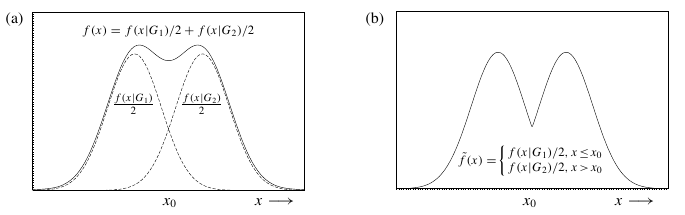
\includegraphics[width=0.8\textwidth]{Pics/Frey1997.png}
\caption{Mixture of two Guassians.}
\label{fig:Frey1997}
\end{figure}

In one-to-many model, we have for each symbol $\vx$ two possible codewords: one given by $G_1$ the other by $G_2$ with the lengths given by $h_{\vx|\vy}(\vx) = -\logb p(\rvx | \rvy = \ry), \ry \in \{1, 2\}$ respecitvely.
Assuming the prior $p(\rvy = 1) = p(\rvy = 2) = 0.5$ we also have $h_{\vy}(1) = h_{\vy}(2) = - \logb 0.5 = 1$ bit to communicate $\rvy$ and hence the identity of the conditional distribution.

A natural choice is to always pick the shorter of the two codewords for $\vx$. This corresponds to a distribution in (b) in \figref{fig:Frey1997} which is clearly suboptimal (gives longer codes then the one-to-one) around $\vx_0$.

\begin{notebox}
Here they show how stochastic one-to-many model relying on the \iterm{bits-back} idea can achieve same rates as the one-to-one scheme.
\end{notebox}

\paragraph{Running example: } We want to encode a symbol $\vx$ that is twice as likely under $G_1$ then $G_2$ so that it requires 2 and 3 bits respectively under the two distributions (that is $p(\vx | \rvy = 1) = 1/4$ and $p(\vx | \rvy = 2) = 1/8$).
With 1 bit to specify the $\rvy$ and hence the conditional distribution we get the total lenght of 3 and 4 bits for the two-level code.
We now have the following options:
\begin{enumerate}[noitemsep, topsep=0pt]
\item picking alwyas the shorter code gives expected length of 3 bits;
\item picking between the two codes equally often (according to the prior $p(\rvy)$) gives expected length of 3.5 bits;
\item use bits-back to get the expected length 2.5 bits.
\end{enumerate}

\begin{notebox}
\paragraph{This is the bits-back idea:}\index{bits-back}
Instead of picking always the shortest codeoword or pick equally often amongst the codeword in the one-to-many setup, you will be picking $\vy \in {1, 2}$ randomly according to some probability $q(\rvy | \rvx)$.
However, to select (sample) $\rvy$ you will use some random sampler based on transorming some auxiliary data $\rvz$ into the samles $\rvy \sim q(\rvy)$.
A trivial example for univariate case is the inverse CDF sampling starting from uniform $\rvz$ or, as they suggest here, the arithmetic decoding which can produce vectorial $\rvy$ starting from a random binary sequence $\rvz$.
Once you sampled $\vy$ you will encode it using $p(\rvy)$ and concatenate with the encoding of $\vx$ using the corresponding $p(\vx | \vy)$.
The message you transmit thus has length $l(\vx, \vy) = - \logb p(\vx | \vy) - \logb p(\vy)$.

The reciever has access to the encoding models $p(\rvy), p(\rvx | \rvy)$ and it 
can thus easily decode the symbols $\rvx$ and $\rvy$ from the codewords $C(\rvx, \rvy)$.
However, it also has access to the sampling distribution $q(\rvy)$ and the algirithm the encoder uses to sample $\rvy$ by transforming $\rvz$.
It can thus reverse this operation (so the transformation must be one-to-one) and recover $\rvz$ at no additional communication cost - these are the `bits-back'.
If $\rvz$ contains some useful information, these `bits-back' essentially reduce the \iterm{effective message length}.
\end{notebox}

In our \textbf{running example} lets imagine $\rvz \in {a, b}$ with $p(\rvz=a)=p(\rvz=b)=0.5$.
Then once we recover $\rvz$ we have communicated $h_{\rvz}(\vz) = - \logb 0.5 = 1$ bit of information at no cost and so the \textbf{expected effective length is $3.5 - 1 = 2.5$ bits}.

How many bits can be recovered is a function of the probability distribution $q(\rvy | \rvx)$.

The \textbf{average code length} for a symol $\vx$ is
\begin{align}
\mathcal{E}(\vx) = \sum_y q(\vy | \vx) l(\vx, \vy) \enspace .
\end{align}
Here $l(\vx, \vy) = - \logb p(\vx | \vy) - \logb p(\vy)$ are the different lengths using different conditionals to encode $\vx$ depending on the choice of $\vy$.

The average information content (the entropy) of the selecting distribution
\begin{align}
\mathcal{H}(\vx) = - \sum_y q(\vy | \vx) \logb q(\vy | \vx)
\end{align}
are \textbf{the average bits back we can recover} for this symbol $\rvx$ when choosing $\vy$ according to $q(\rvy | \vx)$.

\begin{notebox}
This may seem strange cause the symbols we will recover are $\rvz$, not $\rvy$ again.
But since the sampling transformation $f : \rvz \to \rvy$ has to be one-to-one and for the moment \textbf{we assume all the variables are discrete} we heve the trivial result due to prservation of the probability that $q(f(\rvz)) = q(\rvy | \vx)$ (the only thing that happens is re-labelling of the variables) and that the entropy of these two distributions is equal
\begin{align}
\mathcal{H}(\rvx) = - \sum_y q(\vy | \vx) \logb q(\vy | \vx) = - \sum_z q(\vz) \logb q(\vz)
\end{align}
A strange consequence of this that \textbf{I don't yet understand} is that the sampling distribution of $q(\rvz)$ essentially has to be the same as $q(\rvy | \rvx)$.
So the inverse CDF above is probably not a good example.
But this gives potentially room for research :)
\end{notebox}

The average effective codeword length of symbol $\vx$ is the difference between the two above
\begin{align}
\mathcal{F}(\vx) = \mathcal{E}(\vx) - \mathcal{H}(\vx) \enspace .
\end{align}
This is also called the \textbf{\iterm{free energy}} - same concept known from statistical physics.

Next comes the question what $q(\rvy | \vx)$ shall be.
They claim it shall be the Boltzman distribution based on the codeword lengths
\begin{align}
q^*(\vy | \vx) = \frac{2^{-l(\vx, \vy)}}{\sum_{\vy'} 2^{-l(\vx, \vy')}}
\end{align}

\begin{proof}[My proof for Boltzman:]
\begin{align*}
\mathcal{F^*}(\vx) & = \mathcal{E^*}(\vx) - \mathcal{H^*}(\vx)
= \sum_y q^*(\vy | \vx) l(\vx, \vy) + \sum_y q^*(\vy | \vx) \logb q^*(\vy | \vx) \\
& = \sum_y \frac{2^{-l(\rvx, \rvy)}}{\sum_{y'} 2^{-l(\rvx, \rvy')}} \left[l(\rvx, \rvy) + \logb \frac{2^{-l(\rvx, \rvy)}}{\sum_{y'} 2^{-l(\rvx, \rvy')}}\right] 
= l(\rvx, \rvy) - l(\rvx, \rvy) - \logb \sum_{y'} 2^{-l(\rvx, \rvy')} \\
& = - \logb \sum_{y'} 2^{-l(\rvx, \rvy')} = 
- \logb \sum_{y'} 2^{\logb p(\vx, \vy)} =
- \logb \sum_{y'} p(\vx, \vy) = - \logb p(\vx)
\end{align*}
The Boltzman brings the free energy to the same lengths as if one-to-one code with $p(\rvx)$ were used so it is optimal.
\end{proof}

I'd think it shall be the posterior $p(\vy \vert \vx) = p(\vy)p(\vx | \vy) / p(\vx)$.

\begin{proof}[My proof for posterior:]
\begin{align*}
\mathcal{F^*}(\vx) & = \mathcal{E^*}(\vx) - \mathcal{H^*}(\vx)
= \sum_y p(\vy | \vx) l(\vx, \vy) + \sum_y p(\vy | \vx) \logb p(\vy | \vx) \\
& = \sum_y p(\vy | \vx) \left[- \logb p(\vx, \vy) + \logb p(\vy | \vx)\right]
= \sum_y p(\vy | \vx) \left[- \logb p(\vx) \right] = - \logb p(\vx)
\end{align*}
The posterior brings the free energy to the same lengths as if one-to-one code with $p(\rvx)$ were used so it is also optimal.

\begin{notebox}
Does this mean that the Boltzman and the posterior distributions are the same?

\begin{align*}
q^*(\vy | \vx) & = \frac{2^{-l(\vx, \vy)}}{\sum_{\vy'} 2^{-l(\vx, \vy')}}
= \frac{2^{\logb p(\vx, \vy)}}{\sum_{\vy'} 2^{\logb p(\vx, \vy')}} \nn
& = \frac{p(\vx, \vy)}{\sum_{\vy'} p(\vx, \vy')} = \frac{p(\vx, \vy)}{p(\vx)} = p(\vy | \vy)
\end{align*}
So Boltzman baseded on the codeword lengths and the posterior are indeed one and the same thing!
\end{notebox}

$p(\rvy \vert \rvx) p(\rvx) = p(\rvx , \rvy)$ so if we use this to get the codewords we get the lengths $l(\rvx, \rvy) = - \logb p(\rvx , \rvy)$.
Plug this into the free energy
\begin{align*}
\mathcal{F(\rvx)} & = \mathcal{E(\rvx)} - \mathcal{H(\rvx)} = \sum_y p(\rvy | \rvx) l(\rvx, \rvy) + \sum_y p(\rvy | \rvx) \logb p(\rvy | \rvx) \\
& = \sum_y p(\rvy | \rvx) \left[- \logb p(\rvx, \rvy) + \logb p(\rvy | \rvx)\right]
= \sum_y p(\rvy | \rvx) \left[- \logb p(\rvx) \right] = - \logb p(\rvx)
\end{align*}
and we get this is equal to the optimal codelength for the one-to-one code based on $p(\rvx)$.
\end{proof}

In our \textbf{running example} we use the result for the optimal free energy
$\mathcal{F^*}(\vx) = - \logb \sum_{y'} 2^{-l(\rvx, \rvy')}$ with the length
$l(\vx, 1) = 3$ bits and $l(\vx, 2) = 4$ bits we get
$\mathcal{F^*}(\vx) = - \logb (2^{-3} + 2^{-4}) = 2.415$ bits.
This is shorter (better) then the naive sampling used above with $q(\rvy | \vx) = 0.5$ which gave 2.5 bits.

\begin{notebox}
Alternative ways to write the free energy
\begin{align*}
\mathcal{F}(\vx) & = \mathcal{E}(\vx) - \mathcal{H}(\vx)
= \sum_y q(\vy | \vx) l(\vx, \vy) + \sum_y q(\vy | \vx) \logb q(\vy | \vx) \\
& = \sum_y q(\vy | \vx) \logb 2^{l(\vx, \vy)} + \sum_y q(\vy | \vx) \logb q(\vy | \vx) \\
& = \sum_y q(\vy | \vx) \logb \frac{ q(\vy | \vx)}{2^{-l(\vx, \vy)}}
= \sum_y q(\vy | \vx) \logb \frac{ q(\vy | \vx)}{p(\vx, \vy)} \\
& = \sum_y q(\vy | \vx) \logb \frac{ q(\vy | \vx)}{p(\vy | \vx) p(\vx)} 
= \sum_y q(\vy | \vx) \logb \frac{ q(\vy | \vx)}{p(\vy | \vx)}
- \sum_y q(\vy | \vx) \logb p(\vx)
\enspace .
\end{align*}

Here we are quickly getting to ELBO!
Take the expected free energy
\begin{align}
\E_{p(\rvx)} \mathcal{F}(\rvx)
& = \sum_x \sum_y p(\rvx) q(\vy | \rvx) \logb \frac{ q(\vy | \vx)}{p(\vy | \rvx)}
- \sum_x \sum_y p(\vx) q(\vy | \vx) \logb p(\vx) \nn
& = \KL(q(\rvy | \rvx) || p(\rvy | \rvx)) - \E_{p(\rvx)} \logb p(\rvx) = - ELBO
\end{align}

\end{notebox}

How much do we suffer from not using the Boltzman (posterior) $q^*(\vy | \vx) = p(\rvy| \vx)$ but some other distribution $q(\vy | \vx)$ to sample $\rvy$? 
Its the difference in the free energies:
\begin{align*}
\mathcal{F}(\vx) - \mathcal{F^*}(\vx) 
& = \sum_y q(\vy | \vx) l(\vx, \vy) + \sum_y q(\vy | \vx) \logb q(\vy | \vx) + \logb p(\vx) \nn
& = \sum_y q(\vy | \vx) \logb \frac{q(\vy | \vx) p(\vx)}{2^{-l(\vx, \vy)}}
= \sum_y q(\vy | \vx) \logb \frac{q(\vy | \vx) p(\vx)}{p(\vx, \vy)}
= \sum_y q(\vy | \vx) \logb \frac{q(\vy | \vx)}{p(\vy | \vx)}
\end{align*}
This is the KL divergence between the sampling distribution $q(\vy | \vx)$ and the optimal Boltzman or posterior distribution $p(\vy | \vx) = q^*(\vy | \vx)$.


\subsection{Bits-back coding algorithm}

If $\rvy$ is not simply two-valued or diadic (powers of two) variable, they propose to use arithmetic coding as the $f : \rvz \to \rvy$ algorithm.

